\documentclass[journal=jcisd8,manuscript=article]{achemso}
\usepackage{graphicx}
\usepackage{xr-hyper}
\usepackage{hyperref}
\usepackage{xcolor}
\usepackage{verbatim}
\usepackage[subrefformat=parens]{subcaption}
\usepackage[finalizecache,cachedir=.]{minted}
\usepackage[version=3]{mhchem} % Formula subscripts using \ce{}

\renewcommand{\thetable}{S\arabic{table}}  
\renewcommand{\thefigure}{S\arabic{figure}}

\author{Paul G. Francoeur}
\author{David R. Koes}
\email{dkoes@pitt.edu}
\affiliation[Pitt]{Department of Computational and Systems Biology, University of Pittsburgh, Pittsburgh, PA 15260}

\title{Supporting Information:\\SolTranNet -- A ML tool for fast aqueous solubility prediction.}
\begin{document}
\begin{table}
    %\centering
    \begin{tabular}{|c|c|c|c|c|c|c|}
        \hline
         Model & Parameters & CCV $R^2$ & Fold0 $R^2$ & Fold1 $R^2$ & Fold2 $R^2$ & Ind $R^2$ \\
         \hline
         MAT & 42,049,537 & 0.532 & 0.751 & 0.332 & 0.715 & 0.375  \\
         \hline
         0 & 21,061,633 & 0.670 & 0.778 & 0.520 & 0.727 & 0.4718 \\
         1 & 502,529 & 0.662 & 0.769 & 0.465 & 0.733 & 0.4576 \\
         2 & 336,385 & 0.693 & 0.764 & 0.563 & 0.706 & 0.4890 \\
         3 & 336,385 & 0.672 & 0.764 & 0.539 & 0.685 & 0.4461 \\
         4 & 22,657 & \textbf{0.724} & 0.780 & \textbf{0.626} & 0.716 & 0.4831 \\
         5 & 11,905 & \textbf{0.723} & \textbf{0.793} & 0.595 & 0.744 & 0.4628 \\
         6 & 11,905 & 0.713 & 0.786 & 0.582 & \textbf{0.756} & 0.4517 \\
         \emph{7} & \emph{3,393} & \emph{0.6764} & \emph{0.7914} & \emph{0.5243} & \emph{0.7424} & \emph{\textbf{0.5528}}\\
         8 & 2,609 & 0.695 & 0.779 & 0.545 & 0.737  & 0.4589\\
         9 & 2,609 & 0.677 & 0.767 & 0.552 & 0.720  & 0.4678\\
         \hline
         Elastic & 1,463 & 0.414 & 0.441 & 0.394 & 0.408  & 0.377\\
         Lasso & 1,077 & 0.395 & 0.409 & 0.378 & 0.392  & 0.351\\
         PLS & 2,048 & 0.228 & 0.212 & 0.333 & 0.0747  & 0.676\\
         Ridge & 2,048 & 0.319 & 0.289 & 0.354 & 0.291 & 0.261 \\
         \hline
    \end{tabular}
    \caption{SolTranNet hyperparameter search correlations. There is a general trend of models with fewer parameters performing better. Additionally, all models significantly outperform linear ML approaches. The model in italics is the final model selection.}
    \label{tab:solsearchr2}
\end{table}

\begin{table}
    %\centering
    \begin{tabular}{|c|c|}
        \hline
         Index & Description \\
         \hline
         0-11 & Atom Identity as one-hot (B,N,C,O,F,P,S,Cl,Br,I,Dummy,Other) \\
         12-17 & Number of heavy atom neighbors as one-hot of 0-5 \\
         18-22 & Number H atoms as one-hot of 0-4 \\
         23 & Formal Charge \\
         24 & In a Ring \\
         25 & Aromatic \\
         \hline
    \end{tabular}
    \caption{Featurization used to embed atoms in SolTranNet. This is the same schema as in the original MAT implementation. }
    \label{tab:atomembed}
\end{table}


\begin{figure}[tb]
    \centering
    \begin{subfigure}[t]{0.48\textwidth}
        \centering
        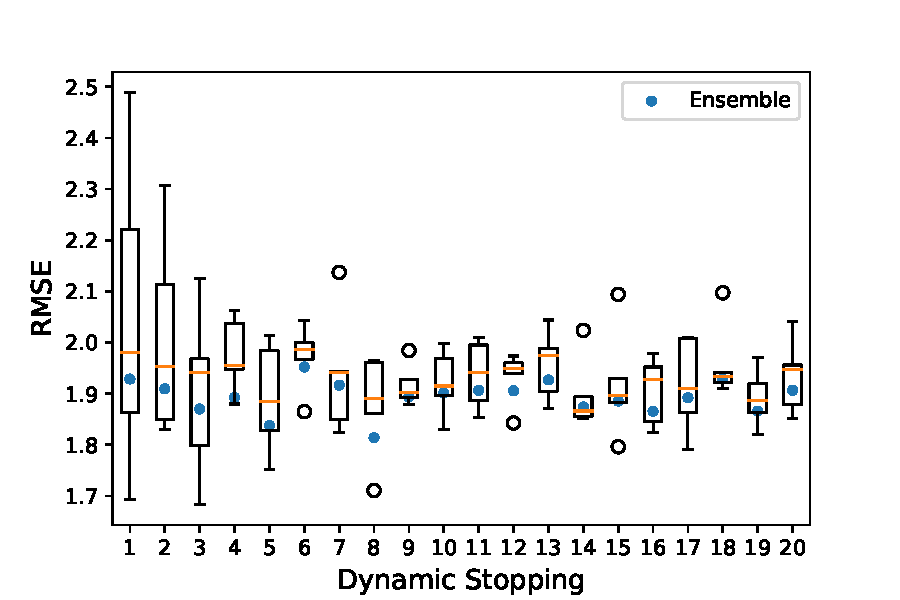
\includegraphics[width=\linewidth]{figures/final_model_ind_dyn_RMSE.pdf}
    \end{subfigure}%
    \hfill
    \begin{subfigure}[t]{0.48\textwidth}
        \centering
        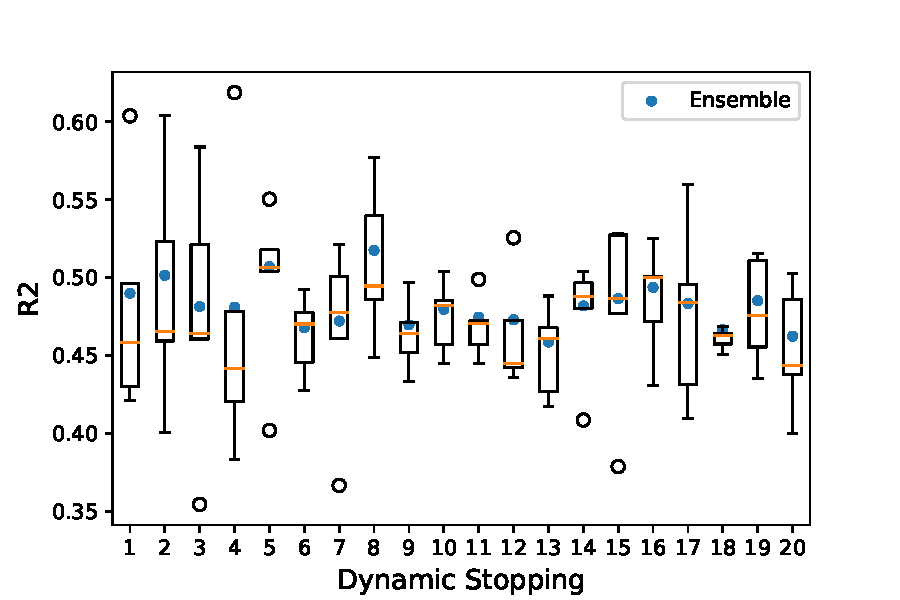
\includegraphics[width=\linewidth]{figures/final_model_ind_dyn_R2.pdf}
    \end{subfigure}
    \caption{Boxplots of the performance of SolTranNet models on our independent test set using various dynamic stopping criteria. The Dynamic Stopping is the number of epochs that the model can fail to improve its fit to the training set before training is stopped. The boxplot is of 5 different seeds, with the ensemble performance shown with the blue dot. Interestingly, the ensemble outperforms the mean performance of the 5 models, but fails to be better than the best performing seed in all cases.}
    \label{fig:dynsweep}
\end{figure}

\begin{figure}[tb]
    \centering
    \begin{subfigure}[t]{0.48\textwidth}
        \centering
        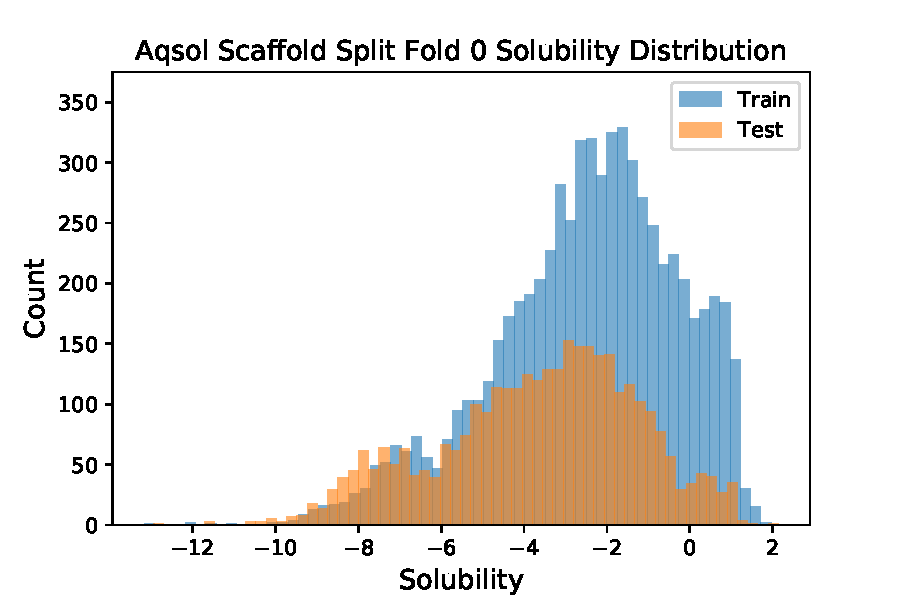
\includegraphics[width=\linewidth]{figures/aqsol_scaf0_soldist.pdf}
    \end{subfigure}%
    \hfill
    \begin{subfigure}[t]{0.48\textwidth}
        \centering
        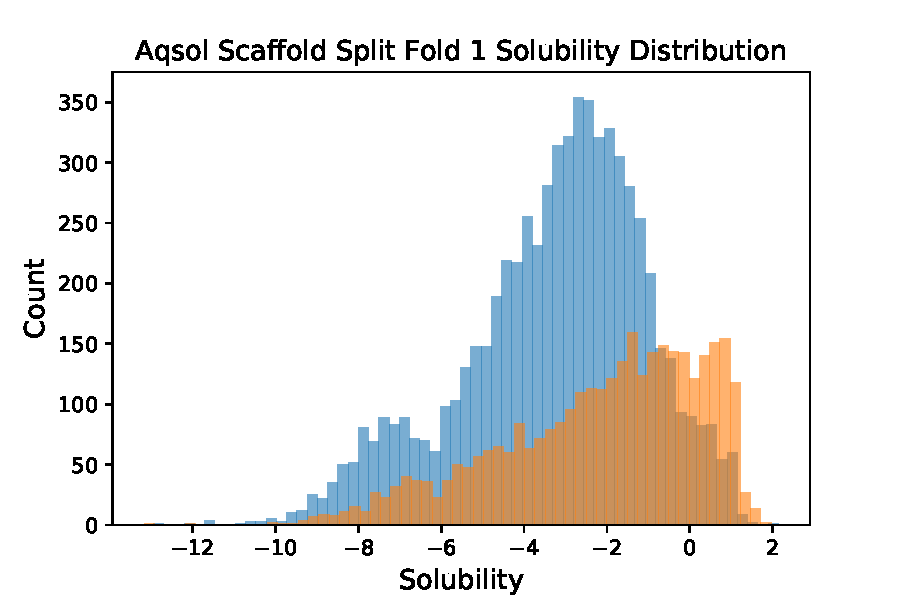
\includegraphics[width=\linewidth]{figures/aqsol_scaf1_soldist.pdf}
    \end{subfigure}
    
    \begin{subfigure}[t]{0.48\textwidth}
        \centering
        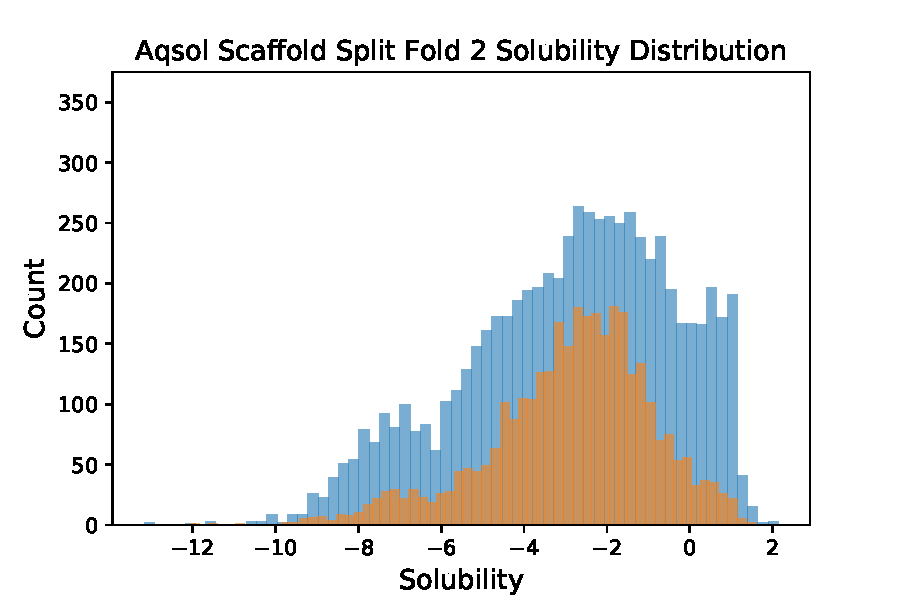
\includegraphics[width=\linewidth]{figures/aqsol_scaf2_soldist.pdf}
    \end{subfigure}
    
    
    \begin{subfigure}[t]{0.48\textwidth}
        \centering
        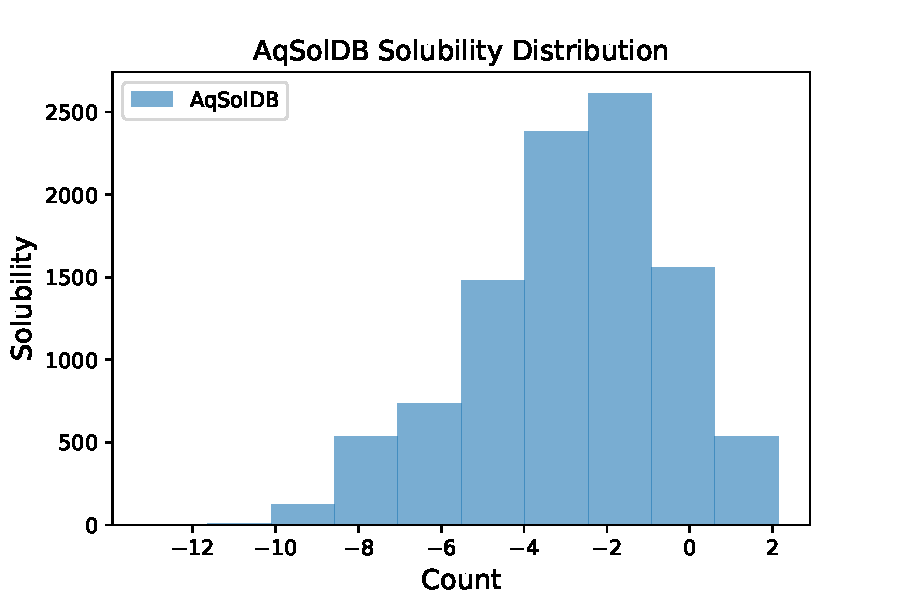
\includegraphics[width=\linewidth]{figures/AqSolDB_solhist.pdf}
    \end{subfigure}%
    \hfill
    \begin{subfigure}[t]{0.48\textwidth}
        \centering
        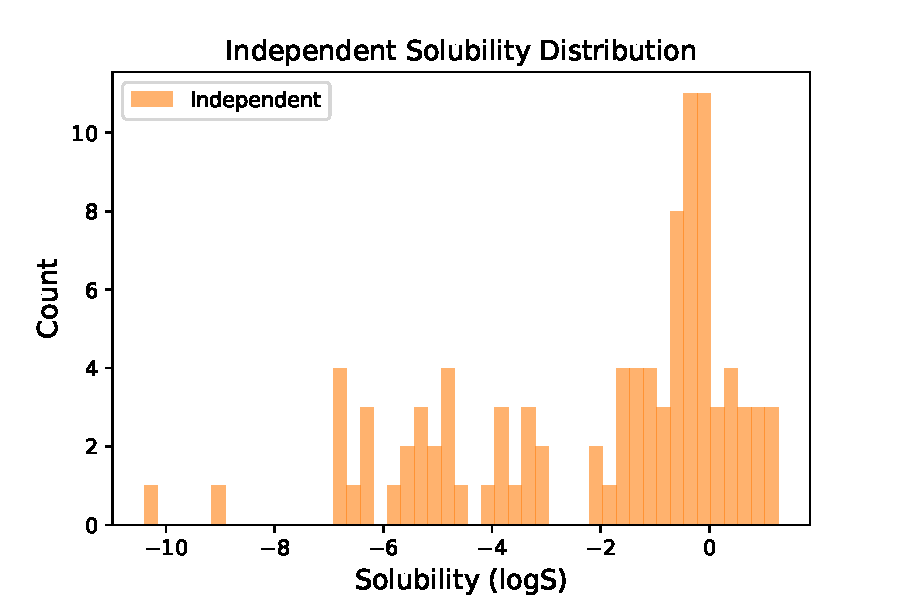
\includegraphics[width=\linewidth]{figures/Independent_solhist.pdf}
    \end{subfigure}
    \caption{Distributions of our various training set data. Each bin has a width of 0.25 units. The first 3 histograms are for the 3 fold scaffold split of AqSolDB, and the last 2 are the full AqSolDB and out independent test set. Note that fold 1 of our scaffold split is particularly challenging as the test set distribution is very different from the training set.}
    \label{fig:solhists}
\end{figure}

\begin{figure}[tb]
    \centering
    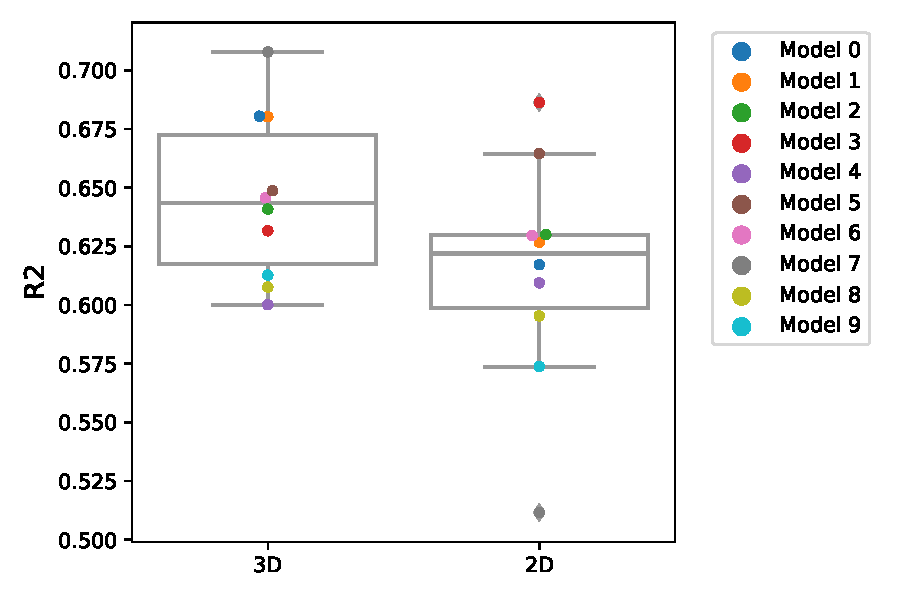
\includegraphics[width=\linewidth]{figures/2dv3d_r2.pdf}
    \caption{$R^2$ performance dependent on if the distance matrix of SolTranNet used 3D conformers of the molecules for the first 10 models we trained in our architecture sweep. There is no statistically significant difference between these two collections ($p=0.116$), but the mean performance of the 3D models is better than the 2D models (0.646 vs 0.614).}
    \label{fig:2dv3dr2}
\end{figure}

\begin{figure}[tb]
    \centering
    \begin{subfigure}[t]{0.48\textwidth}
        \centering
        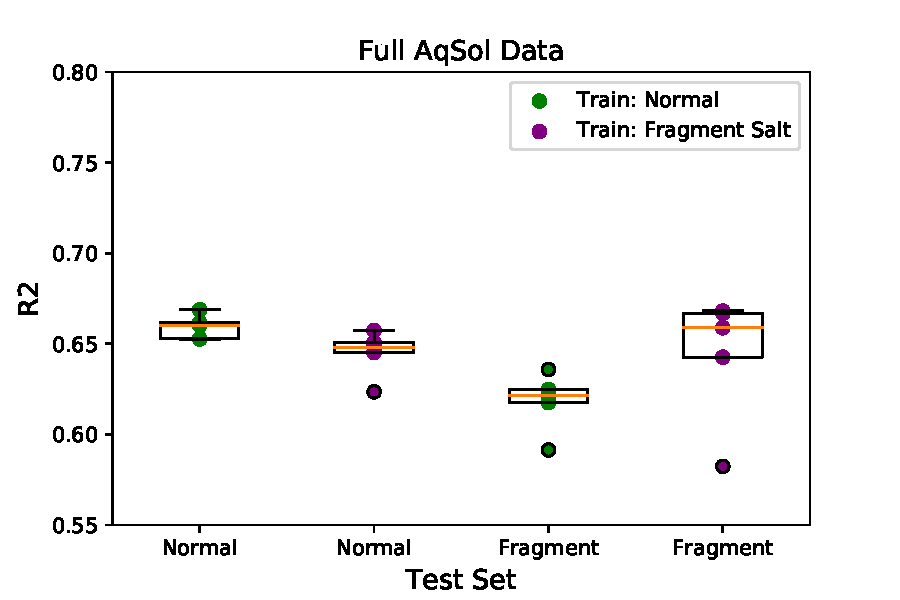
\includegraphics[width=\linewidth]{figures/full_saltfragfirst_R2s_boxplots.pdf}
        \caption{No statistically significant difference between performance on either test set when comparing training with or without fragmented salts ($p=$0.0596 and 0.1852).}
        \label{fig:fullsfr2}
    \end{subfigure}%
    \hfill
    \begin{subfigure}[t]{0.48\textwidth}
        \centering
        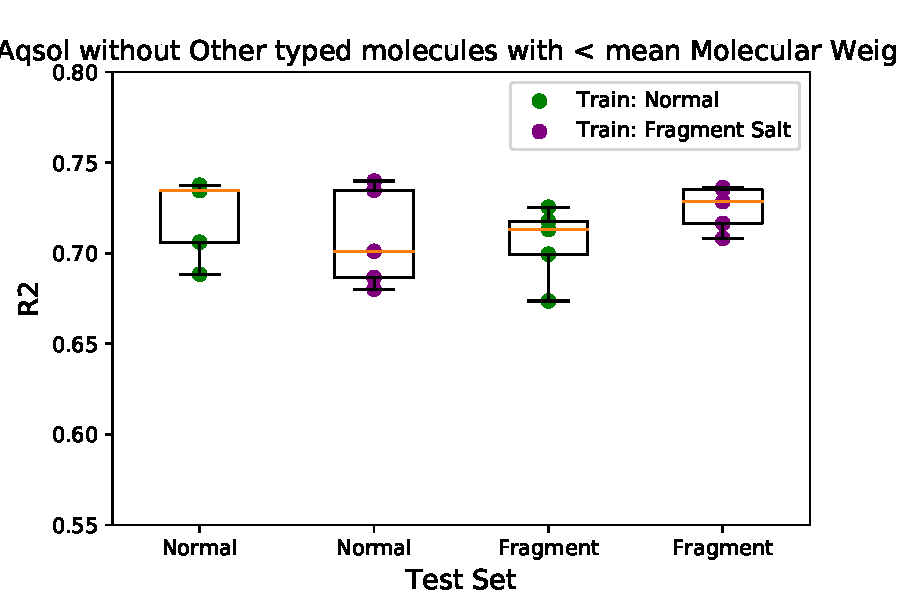
\includegraphics[width=\linewidth]{figures/othersMW_saltfragfirst_R2s_boxplots.pdf}
        \caption{No statistically significant difference between performance on either test set when comparing training with or without fragmented salts ($p=$0.4751 and 0.1100).}
        \label{fig:mwsfr2}
    \end{subfigure}
    
    \begin{subfigure}[t]{0.48\textwidth}
        \centering
        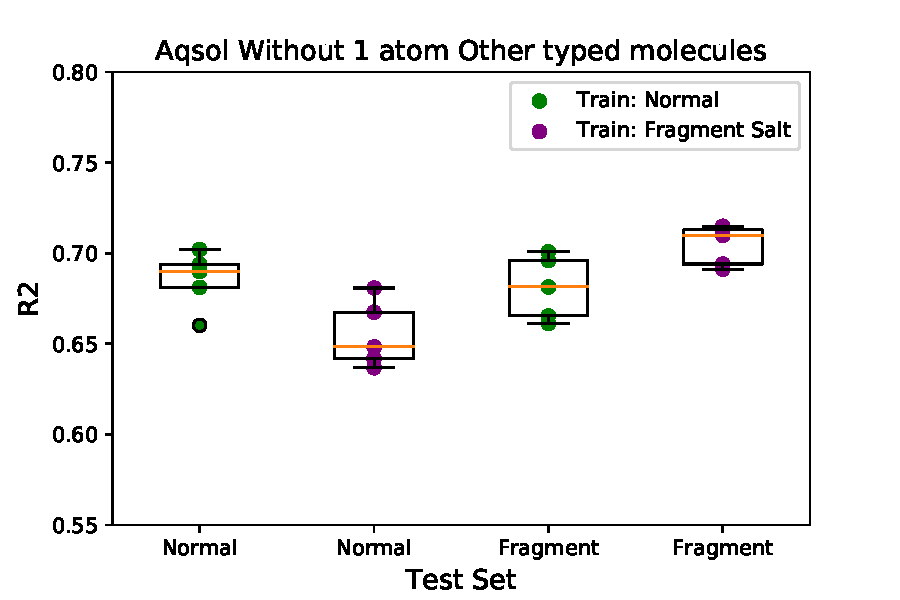
\includegraphics[width=\linewidth]{figures/others2plus_saltfragfirst_R2s_boxplots.pdf}
        \caption{Training with fragmenting salts performed worse on testing on Normal ($p=0.0240$) and better on testing on Fragment ($p=0.03547$).}
        \label{fig:onesfr2}
    \end{subfigure}%
    \hfill
    \begin{subfigure}[t]{0.48\textwidth}
        \centering
        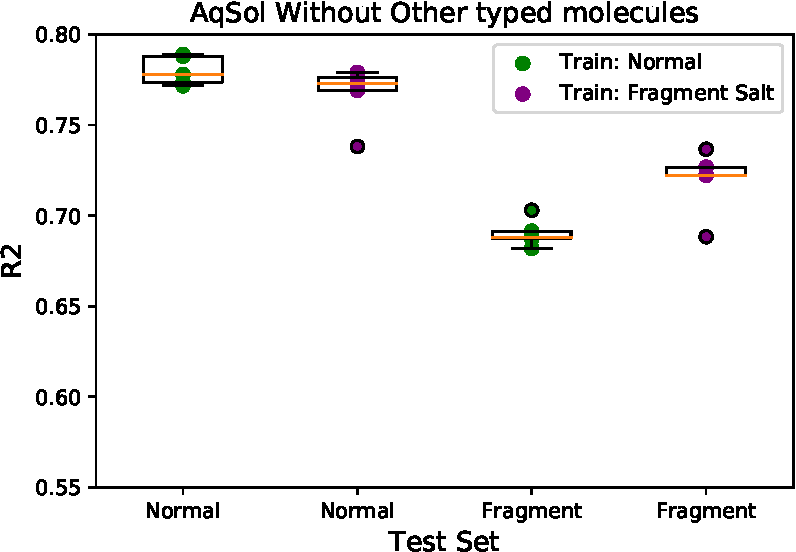
\includegraphics[width=\linewidth]{figures/noothers_saltfragfirst_R2s_boxplots.pdf}
        \caption{Training with fragmented salts had no effect on testing on Normal ($p=0.1555$), but performed better when testing on Fragment ($p=0.0116$).}
        \label{fig:noothersdf2}
    \end{subfigure}
    \caption{$R^2$ of 5 different SolTranNet trained on the scaffold split of AqSolDB. The horizontal axis is dependent on if the salts were fragmented in the test set, while the colors of the boxplot are dependent on if the salts were fragmented in the training set. Each plot has successively fewer data points in the training and testing sets by more stringently removing atoms which would be embedded as ``Other type'' during training.}
    \label{fig:saltfragr2}
\end{figure}


\begin{table}
    \begin{tabular}{|c|c|c|c|c|c|}
        \hline
         Dataset & Reported $R^2$ & STN Training $R^2$ &  STN Best $R^2$ & STN Deployed $R^2$ & Overlap \\
        \hline
         Cui2020 & 0.412 & 0.589(0.0244) & 0.611 &  0.656 & 0/62 \\
        Boobier2017 & 0.706 &  0.543(0.142) & 0.724 &  0.773 & 23/25 \\
        Louvric2020 &  -- & 0.709(0.0537) & 0.783 & 0.744(0.0345) & 151.4/166 \\
        Llinas2020 set1 & 0.62 & 0.496(0.0268) &  0.527 & 0.514 & 79/100 \\
        LLinas2020 set2 & 0.75 & 0.769(0.0346) & 0.824 & 0.726 & 18/32 \\
        \hline
    \end{tabular}
    \caption{Performance of SolTranNet (STN) on other published datasets. For SolTranNet training, we trained 5 different seeds of our final architecture on the provided training and testing splits and report the mean and standard deviation. The SolTranNet Deployed column is using our final deployed model to predict the provided test set. The final column is the overlap of the provided test set with our deployed model's training set. Notably the Louvric set had 5 different randomly selected splits for training and testing, which is why there is a mean in the Deployed and Overlap columns.}
    \label{tab:othersetsr2}
\end{table}

\end{document}